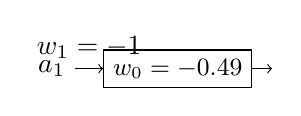
\begin{tikzpicture}[scale=0.4]
	\draw node (w1) {$a_1$} ++(4,0) node[draw] (centro) {\small{$w_0=-0.49$}};
	%\node[init] (centro) {Centro};
	%\node[init, left of=centro] (w1) {$w1$};
	%\node[init] (s2) {$w2$};

	\draw[->] (w1) -- (centro) node[midway,above,sloped] {$w_1=-1$};
	\draw[->] (centro) -- ++(3,0);
\end{tikzpicture}

